\chapter{Field-programmable gate arrays}
\label{cap-fpga}

\section{Introducción}

Las \emph{field-programmable gate arrays} (FPGAs) son dispositivos basados en una matriz de bloques lógicos configurables (CLBs) conectados vía interconexiones programables.
Las FPGAs pueden ser reprogramadas para cualquier aplicación o funcionalidad requerida mientras se encuentre dentro de las limitaciones de la placa. Esta característica las diferencia de las \emph{application specific integrated circuits} (ASICs), las cuales son diseñadas específicamente para ciertas tareas.

En este capítulo se explican distintas características de este tipo de dispositivos, así como los entornos de desarrollos que alrededor de ellos. Primero, se detalla su arquitectura y los bloques elementales que lo conforman, para después informar al lector de los particulares lenguajes de programación utilizados para su programación y los paradigmas en los que se basan. Por último, se enumeran distintas herramientas de software que se emplean para su programación. 

\section{Arquitectura}

Los FPGAs modernos poseen grandes recursos de bloques lógicos y de RAM para implementar calculos complejos, y también periféricos como conversores analógicos-digitales (ADCs) y conversores digitales-analógicos (DACs). La arquitectura básica de un FPGA puede observarse en la Figura \ref{fpga}, la cual consiste de un arreglo de CLBs, pads de entrada/salida (I/O), y canales de enrutamiento.

\begin{figure}[hbt!]
    \centering
    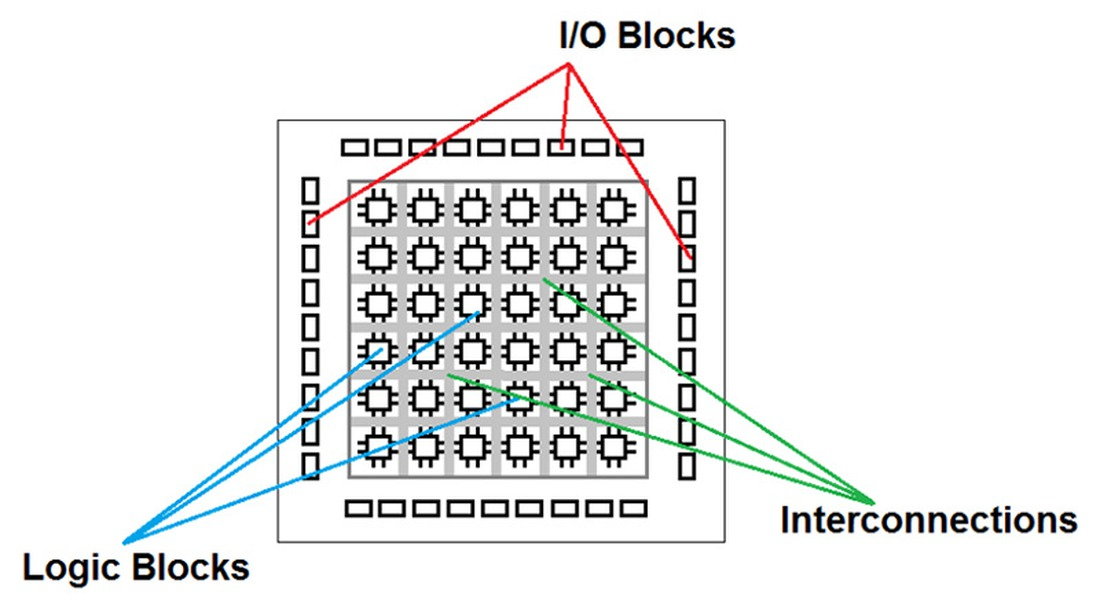
\includegraphics[width=0.45\columnwidth]{Imágenes/Arquitectura de un FPGA.png}
    \caption{Arquitectura básica de un FPGA.}
    \label{fpga}
\end{figure} 

\subsection{Bloques lógicos}

Generalmente, los bloques lógicos de un FPGA consisten de algunas celdas lógicas (llamadas ALM, LE, slices, etc.). Típicamente, estas celdas consisten en una \emph{lookup table} (LUT) con 4 entradas, un \emph{full adder} (FA), y un flip-flop tipo D (DFF). Estos bloques lógicos poseen distintos modos los cuales le otorgan flexibilidad a la hora del uso de sus componentes, y por lo tanto amplía sus funcionalidades. Por ejemplo, en la Figura \ref{clb} puede observarse una celda lógica, perteneciente a un CLB. En ella, hay LUTs de 3 entradas, las cuales mediante un multiplexor, pueden ser combinadas para conseguir una LUT de 4 entradas. Además, la salida de estas celdas lógicas puede ser sincrónicas o asincrónicas, decisión dictada por otro multiplexor.

\begin{figure}[hbt!]
    \centering
    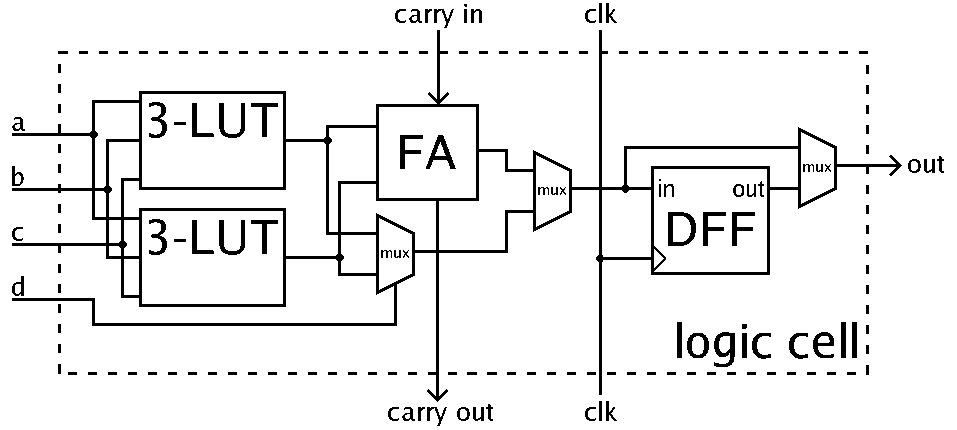
\includegraphics[width=0.65\columnwidth]{Imágenes/Celda lógica de CLB.png}
    \caption{Ilustración simplificada de una celda lógica.}
    \label{clb}
\end{figure} 

\subsection{Integración}
\label{subseccion-nexys-3}

Actualmente, estos bloques lógicos e interconexiones de los FPGAs tradicionales son combinados con microprocesadores embebidos y otros bloques de funcionalidad de alto nivel (multiplicadores, bloques de procesamiento de señales, memorias embebidas, etc.) para formar un \emph{system on chip} (SoC). Un ejemplo de este nuevo enfoque de las FPGAs puede verse en la Figura \ref{spartan6}.   

\begin{wrapfigure}{l}{0.5\textwidth}
    \vspace{-0pt}
    \begin{center}
      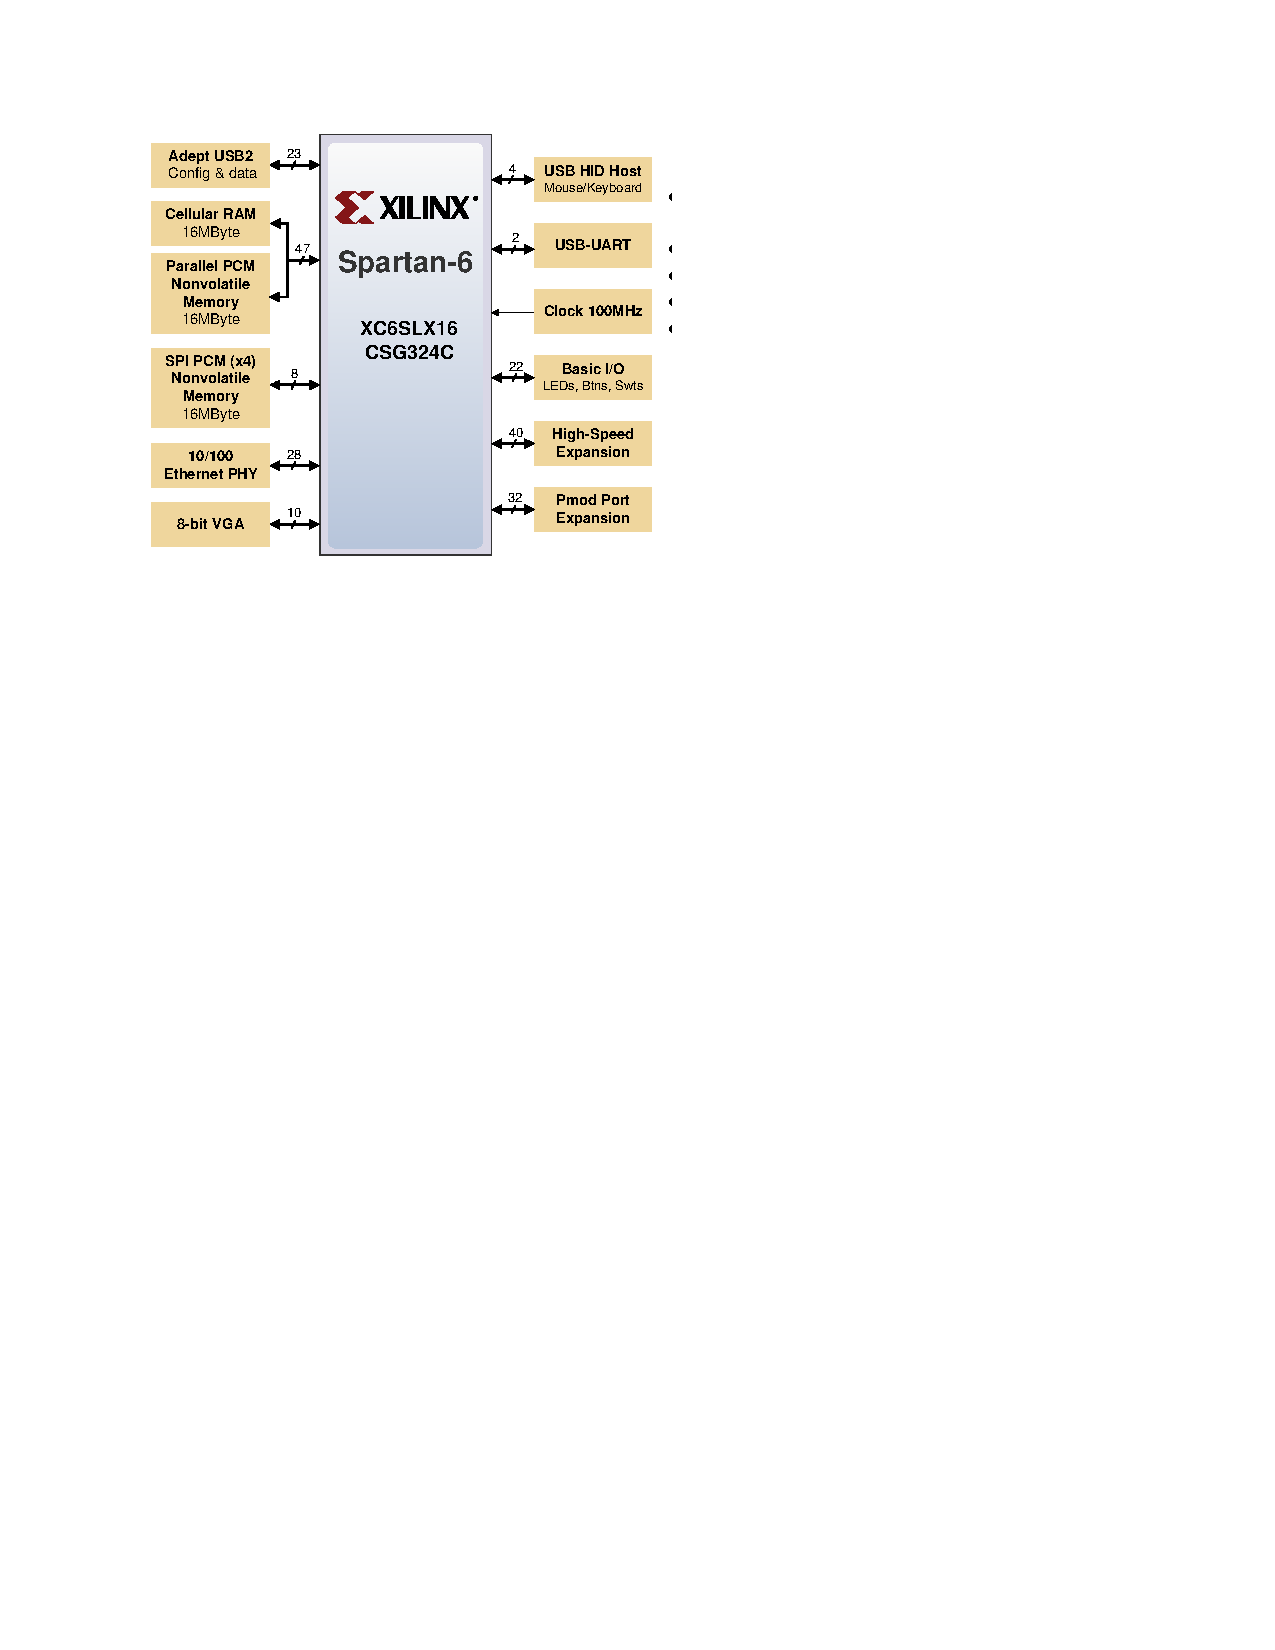
\includegraphics[width=0.41\textwidth]{Imágenes/SoC del Nexys 3.pdf}
    \end{center}
    \caption{Spartan-6 de Xilinx en la placa de desarrollo Nexys 3.}
    \label{spartan6}
  \end{wrapfigure}

Aqui, se puede observar un diagrama de conexionado del FPGA Spartan-6, utilizado en la placa de desarrollo Nexys 3. Además de poseer varios tipos de conexiones, el Spartan-6 posee 2278 \mbox{\emph{slices}} o celdas lógicas, en las cuáles cada una posee cuatro LUTs de 6 entradas y ocho flip-flops. Además, posee 576 kB de RAM, 32 slices enfocados a DSP, y velocidades de reloj de más de \SI{500}{\mega\hertz}. 

A su vez, la placa de desarrollo amplía aún más sus funcionalidades, brindando una colección mejorada de periféricos, como por ejemplo un puerto USB-UART, 16MB de RAM, y 10/100 Ethernet PHY, entre otros \cite{nexys3}.

Esto deja en claro que el objetivo de las FPGAs es proveer flexibilidad a la hora de su uso, brindando una gran variedad de herramientas para cualquier aplicación. Por eso mismo es que este tipo de circuitos es ideal para desarrollar prototipos en las fases iniciales de un proyecto.

\section{Lenguajes de descripción de hardware}

Los lenguajes de descripción de hardware (HDL) son lenguajes de programación utilizados para describir la estructura y comportamiento de circuitos lógicos digitales. Este tipo de lenguajes permite la síntesis de una descripción por HDL a una \emph{netlist} (interconexión de componentes electrónicos físicos descriptos), la cual puede ser implementada para finalmente crear un circuito integrado.

Los HDLs forman una parte íntegra de la automatización de diseño electrónico (EDA, del inglés \mbox{\emph{electronic design automation}}), especialmente para circuitos complejos, y son los lenguajes utilizados en la programación de los FPGAs. Los dos lenguajes más utilizados son Verilog, y VHDL.

\subsection{Verilog}

En Verilog, el diseño consiste de una jerarquía de módulos. Estos módulos son definidos con conjuntos de puertos de entrada, salida y bidireccionales. Internamente, un módulo contiene una lista de cables y registros. Las sentencias concurrentes y secuenciales definen el comportamiento del módulo, describiendo las relaciones entre los puertos, cables, y registros. Las sentencias secuenciales son colocadas dentro de un boque \texttt{begin}/\texttt{end} y ejecutadas en orden secuencial, pero todas las sentencias concurrentes y todos los bloques \texttt{begin}/\texttt{end} son ejecutados en paralelo en el diseño. Un módulo puede contener una o más instancias de otro módulo para definir un subcomportamiento.

Un subconjunto de sentencias en el lenguaje es sintetizable. Si los módulos en un diseño contienen sólo sentencias sintetizables, puede ser sintetizado en una \emph{netlist} que describe los componentes básicos y los conectores que deben implementarse en hardware. La \emph{netlist} o lista de nodos puede ser entonces convertido en un \emph{bitstream} para programar el FPGA.

\subsection{VHDL}

VHDL (acrónimo de \emph{Very High Speed Hardware Description Language} en inglés) es un HDL que hereda muchos conceptos de lenguajes de programación a alto nivel (por ejemplo C o PASCAL). Una característica importante heredada es el concepto de tipos de datos. Por ejemplo, los tipos de datos \emph{bit}, \emph{boolean}, \emph{integer}, etc. ya se encuentran incorporados, pero existe la posibilidad de definir nuevos tipos, como por ejemplo matrices, registros, o punteros. Esto permite una programación a un distinto nivel de atracción.

Otra característica no menor es la del control de flujo, incorporando condicionales (\emph{if}, \emph{case}) e iteraciones (\emph{for}, \emph{while}). Además, es posible estructurar o modularizar el código, ya que se pueden agrupar partes del código en subprogramas en funciones (\emph{function}) o procedimientos (\emph{procedures}), e incluye la posibilidad de desarrollar y utiliza bibliotecas de diseño.

Aunque varias características son heredadas de otros lenguajes de programación, VHDL es un HDL en sí, y por lo tanto es necesario explicar sus conceptos específicos para modelado de hardware.

\subsubsection{Modelo de estructura}
\label{vhdl-estruct}

Cualquier sistema electrónico puede dividirse en subsistemas más pequeños hasta llegar a su nivel primitivo (es decir, al nivel de puertas lógicas). Por eso mismo VHDL incorpora el concepto de estructura. Esta característica nos permite realizar el modelo de un sistema digital cualquier a partir de la referencia a las distintas partes que lo forman, especificando la conexión entre éstas. Cada una de las partes, a su vez, pueden estar modeladas de forma estructural a partir de sus componentes, o bien estar descritas de forma funciona, utilizando los conceptos heredados de los lenguajes de programación de alto nivel. En el nivel más alto de jerarquía se encuentran los modelos funcionales, a partir de los cuales se construye el sistema completo.

\begin{wrapfigure}{r}{0.45\textwidth}
  \vspace{-20pt}
  \begin{center}
    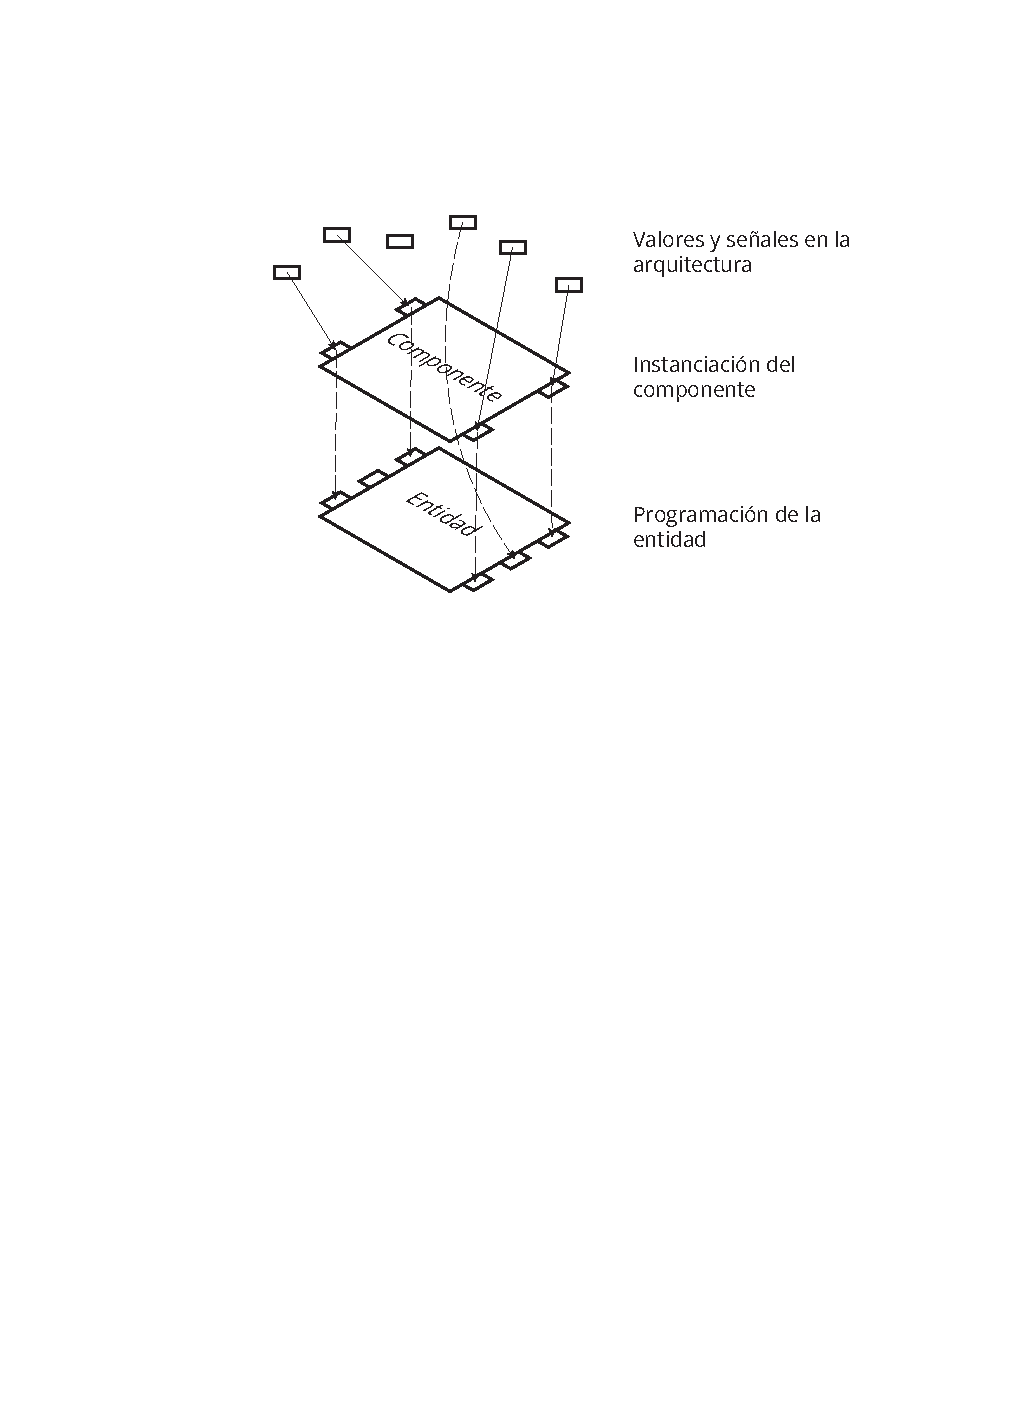
\includegraphics[width=0.41\textwidth]{Imágenes/Asociación entidad-componente.pdf}
  \end{center}
  \caption{Asociación entidad-componente-arquitectura de un modelo.}
  \label{entidad-componente}
\end{wrapfigure}

En la descripción de un dispositivo en VHDL, el diseñador debe definir dos elementos principales: la interfaz del dispositivo con el exterior (\emph{entity}) y la descripción de la funcionalidad que realiza el dispositivo \mbox{(\emph{architecture}}). La interfaz de un dispositivo tiene por objeto definir qué señales del dispositivo son visibles o accesibles desde el exterior, llamados puertos (\emph{ports}) del dispositivo. En la arquitectura se definirá la funcionalidad que implementa dicho dispositivo respecto de lo datos ingresantes a los puertos de entrada, para producir nuevos valores sobre los puertos de salida.

En la Figura \ref{entidad-componente} se representa gráficamente la asociación de una interfaz de un dispositivo a partir de la instanciación de un componente con los valores y señales de una arquitectura en donde es invocado.

VHDL además permite la instanciación de estos dispositivos a partir del concepto de componente (\emph{component}) y de referencia a un componente. Cualquier elemento modelado en VHDL puede ser utilizado como un componente de otro diseño, y para ello solamente es necesario hacer referencia al elemento a utilizar y conectar los puertos de su interfaz a los puntos necesarios para realizar el nuevo diseño.

El diseñador sólo debe preocuparse de las entradas y salidas de los subsistemas (es decir, su interfaz), y de la forma adecuada en que debe realizar su conexión bajo su modelo, pero no es necesario conocer cómo está descrito cada uno de los subsistemas.


\subsubsection{Modelo de concurrencia}

El hardware es por definición \emph{concurrente}\footnote{La concurrencia es la habilidad de diferentes partes de un algoritmo o programa de ser ejecutados fuera de orden o en un orden parcial, lo que permite su ejecución en paralelo.}, y en su última instancia cualquier dispositivo digital está formado de un mar de puertas lógicas, todas ellas funcionando en paralelo. El elemento básico que ofrece VHDL para modelar el paralelismo es el proceso (\emph{process}).

En general, el código que describe un proceso se ejecuta en forma secuencial, pero todos los procesos se ejecutarán en paralelo.

Estos procesos que se ejecutan concurrentemente deben poder comunicarse (sincronizarse) entre ellos. El elemento utilizado para esta vinculación es la señal (\emph{signal}). Cada proceso tiene un conjunto de señales a la que es sensible, lo que significa que el proceso se ejecuta cuando se produce un cambio o evento de dicha señal. La ejecución del proceso, el cual es un bucle infinito, puede ser suspendida con la sentencia \emph{wait}.

\subsubsection{Modelo de tiempo}

Una de las finalidades del modelado en VHDL del hardware es poder observar su comportamiento a lo largo del tiempo en una simulación o \emph{test bench}. Esto implica que las construcciones del lenguaje tendrán asociada una semántica respecto a la simulación, es decir, influirán en ésta provocando distintos eventos que sucederán a lo largo del tiempo, y a su vez, el modo en que se comportan las sentencias dependerá de los eventos que se sucedan a lo largo de la simulación.

Entonces, la simulación o \emph{test bench} de un modelo VHDL es una simulación dirigida por eventos. Esto significa que el simulador mantiene unas listas de eventos (cambios en las señales internas del modelo y también de las entradas y salidas) que se han de producir a lo largo del tiempo de simulación. Como el comportamiento del modelo es estable mientras no se produzca un evento, la tarea del simulador consiste en avanzar el tiempo de simulación hasta el siguiente evento y calcular sus consecuencias sobre la lista de eventos futuros.

Normalmente la reacción del modelo a un evento ocasionará la ejecución de otros eventos en un tiempo de simulación posterior que se añadirán a la lista. La simulación finaliza cuando se ha alcanzado el tiempo de simulación especificado por el usuario o cuando no existen más eventos.

\section{Entornos de desarrollo} 
\label{desarrollo-fpga}

\subsection{Intel Quartus Prime}

\emph{Intel Quartus Prime}\textsuperscript\textregistered\hspace{0.05pt} es el entorno de diseño desarrollado por Intel\textsuperscript\textregistered\hspace{0.05pt} (previamente por Altera). Permite al usuario el análisis y síntesis de diseños HDL, lo que habilita al desarrollador a compilar sus diseños, realizar análisis de tiempo, examinar diagramas RTL, simular la reacción de un modelo frente a distintos estímulos, y configurar el dispositivo a utilizar con el programador. Es importante aclarar que esto último solamente es posible con familias de FPGAs que Quartus Prime\textsuperscript\textregistered\hspace{0.05pt} soporta, como por ejemplo la familia \emph{Cyclone}.
Quartus Prime\textsuperscript\textregistered\hspace{0.05pt} incluye una implementación de VHDL y Verilog para descripción de hardware, edición visual de circuitos lógicos, y simulación de formas de onda vectoriales.

\subsection{Xilinx ISE}

\emph{Xilinx ISE}\textsuperscript\textregistered\hspace{0.05pt} (\emph{Integrated Synthesis Environment}) es una herramienta de software de Xilinx\textsuperscript\textregistered\hspace{0.05pt} para la síntesis y análisis de diseños HDL, la cual está principalmente dirigida al desarrollo de las familias de productos de FPGAs de Xilinx\textsuperscript\textregistered\hspace{0.05pt} (por ejemplo, Spartan-6).

Posee las mismas funcionalidades descritas anteriormente para \emph{Intel Quartus Prime\textsuperscript\textregistered\hspace{0.05pt}}, pero además incluye otros componentes, como el \emph{Embedded Development Kit (EDK)}, \emph{Software Development Kit (SDK)}, y \emph{ChipScope Pro}. Por último, también incluye software que permite la simulación y \emph{test bench} del código, como \emph{ModelSim} e \emph{ISim}, los cuales son utilizados en el presente trabajo para verificar la correcta implementación de los algoritmos de control a lo largo del Capítulo \ref{implementacion-control}.

La interfaz de usuario principal del ISE es el \emph{Project Navigator}, el cual incluye la jerarquía de diseño (\emph{sources}), un editor de código (\emph{workplace}), una consola de salida (\emph{transcript}), y un árbol de procesos (\emph{processes}).

La jerarquía de diseño consiste en archivos de diseño (módulos), cuyas dependencias son interpretadas por el ISE y presentadas con una estructura de árbol. Para los diseños de chip único puede haber un módulo principal, con otros módulos incluidos en este, similar a la subrutina \texttt{main()} en programas C++.

Actualmente, Xilinx ISE\textsuperscript\textregistered\hspace{0.05pt} fue descontinuado a favor de \emph{Vivado Design Suite}\textsuperscript\textregistered\hspace{0.05pt}, el cual posee el mismo rol que ISE con características adicionales para el desarrollo de SoCs. Xilinx\textsuperscript\textregistered\hspace{0.05pt} publicó la última versión en octubre de 2013 (versión 14.7) y no se prevén más actualizaciones. 


\section{Resumen}

En este capítulo fue presentada la arquitectura FPGA junto a dos de los lenguajes de programación de hardware más populares para su programación, como a su vez herramientas de su entorno de desarrollo que permiten sintetizar y compilar el código creado para tanto FPGAs de Xilinx\textsuperscript\textregistered\hspace{0.05pt} como Intel\textsuperscript\textregistered\hspace{0.05pt}.

En capítulos posteriores se podrán ver ciertas de estas herramientas en acción, al querer implementar el sistema de control diseñado.